\documentclass[17pt]{flash}
\usepackage{texmaths-tikz}
\usepackage{texmaths-symbols}
\startdatakeys
\cycle{4}
\competencesDuSocle{CH,RA}
\connaissancesRequises{D2b5}
\competencesTravaillees{D2d*}
\motsCles{CAC}
\enddatakeys
\begin{document}

\def\figFont{\footnotesize}

\flashvisibletimertrue
\FlashSetItemSep{0pt}
\FlashSetVtop{-4em}
\FlashSetTitle{}
\FlashShowConsignes{%
    \item Écrire un maximum d'égalités de longueurs.
}

\flash{180}{\figFont
    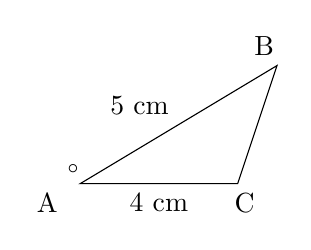
\begin{tikzpicture}[baseline=(current bounding box.center)]
        \coordinate[label=below left:\mathspoint{A}](A)at(0,0);
        \coordinate[label=above:\mathspoint{B}](B)at(2.5,1.5);
        \coordinate[label=below right:\mathspoint{C}](C)at(2,0);
        \tkzFillAngle[size=1](C,A,B)
        \tkzLabelAngle[pos=1.4](C,A,B){\figFont30$^\circ$}
        \path(A)--(C)node[pos=0.5, below]{4 cm};
        \path(A)--(B)node[pos=0.5, above left]{5 cm};
        \draw(A)--(B)--(C)--cycle;
    \end{tikzpicture}
    \begin{tikzpicture}[baseline=(current bounding box.center)]
        \coordinate[label=below left:\mathspoint{G}](A)at(0,0);
        \coordinate[label=above:\mathspoint{H}](B)at(1.5,2);
        \coordinate[label=below right:\mathspoint{J}](C)at(2,0);
        \tkzMarkSegments[mark=s||,colored](A,B A,C)
        \draw(A)--(B)--(C)--cycle;
    \end{tikzpicture}
    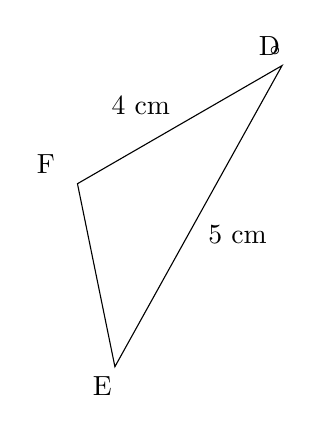
\begin{tikzpicture}[rotate=-150,scale=1.5, baseline=(current bounding box.center)]
        \coordinate[label=above:\mathspoint{D}](A)at(0,0);
        \coordinate[label=below:\mathspoint{E}](B)at(2.5,1.5);
        \coordinate[label=above left:\mathspoint{F}](C)at(2,0);
        \tkzFillAngle[size=1,fill=\currentcolor](C,A,B)
        \tkzLabelAngle[pos=1.2](C,A,B){\figFont30$^\circ$}
        \path(A)--(C)node[pos=0.5, above left]{4 cm};
        \path(A)--(B)node[pos=0.5, below right]{5 cm};
        \draw(A)--(B)--(C)--cycle;
    \end{tikzpicture}
}

\FlashCorrection

\end{document}